\documentclass{standalone}
\usepackage{tikz}
\usepackage{ctex,siunitx,upgreek}
\setCJKmainfont{Noto Serif CJK SC}
\usepackage{tkz-euclide}
\usepackage{amsmath,amsfonts,amssymb}
\usetikzlibrary{patterns, calc,3d}
\usetikzlibrary {decorations.pathmorphing,decorations.pathreplacing,decorations.shapes}
\tikzset{label style/.append style={font=\small}}
\begin{document}
\small
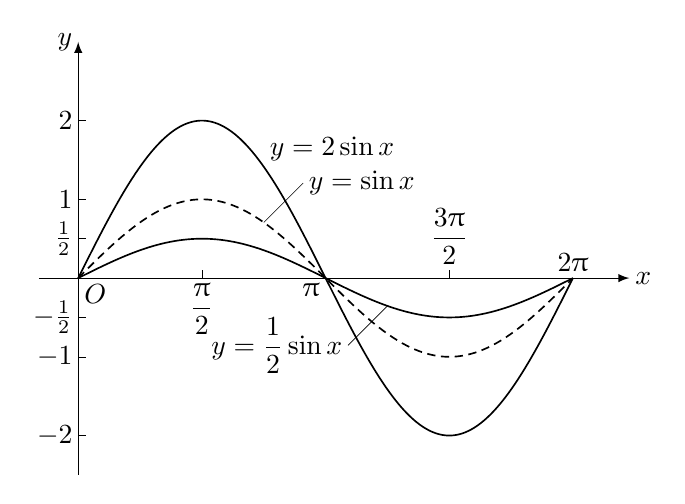
\begin{tikzpicture}[>=latex,scale=1.0,inner sep=2pt]
  \draw[->](-0.5,0)--(7,0)node[right]{$x$};
  \draw[->](0,-2.5)--(0,3)node[left]{$y$};
  \node at (0,0)[below right]{$O$};
  \draw[semithick,densely dashed,samples=200,domain=0:2*pi]plot(\x,{sin(\x r)});
  \draw[semithick,samples=200,domain=0:2*pi]plot(\x,{0.5*sin(\x r)});
  \draw[semithick,samples=200,domain=0:2*pi]plot(\x,{2*sin(\x r)});
  \draw[very thin](0.5*pi,0)node[below]{$\dfrac\uppi2$}--++(0,0.1);
  \draw[very thin](1.5*pi,0)--++(0,0.1)node[above]{$\dfrac{3\uppi}{2}$};
  \node at (pi,0)[below left]{$\uppi$};
  \node at (2*pi,0)[above]{$2\uppi$};
  \draw [very thin](0,2)node[left]{$2$}--++(0.1,0);
  \draw [very thin](0,1)node[left]{$1$}--++(0.1,0);
  \draw [very thin](0,0.5)node[left]{$\frac12$}--++(0.1,0);
  \draw [very thin](0,-0.5)node[left]{$-\frac12$}--++(0.1,0);
  \draw [very thin](0,-1)node[left]{$-1$}--++(0.1,0);
  \draw [very thin](0,-2)node[left]{$-2$}--++(0.1,0);
  \draw [very thin](0.75*pi,0.707)--++(0.5,0.5)node[right]{$y=\sin x$};
  \draw [very thin](1.25*pi,-0.354)--++(-0.5,-0.5)node[left]{$y=\dfrac12\sin x$};
  \node at (0.75*pi,1.414)[above right]{$y=2\sin x$};
\end{tikzpicture}
\end{document}